\chapter{Discusión de Resultados}
\label{chap:discusion-resultados}

\lettrine{E}{ste} capítulo realiza una comparación de todas las
técnicas implementadas a lo largo del trabajo:
\gls{htn} (Capítulo~\ref{chap:iter1}), \gls{il}
(Capítulo~\ref{chap:iter2}) y \gls{rl} (Capítulo~\ref{chap:iter3}).
Todas ellas entrenadas y evaluadas sobre la misma tarea y bajo una métrica común 
de tasa de éxito: talar $k=\num{5}$ troncos. 

Si bien en cada capítulo se analizan en profundidad los resultados de cada implementación, 
este capítulo pretende generar un análisis más general comparando todas las familias. 

\section{Metodología de Evaluación}
\label{sec:eval-metodologia}
Todas las técnicas se evalúan bajo las mismas condiciones para que la comparación sea justa.
Cada agente ejecuta \textbf{\num{50} episodios} en el mismo mundo, con un \textbf{punto de
aparición fijo} y distinto del usado en el entrenamiento, de modo que ninguna
técnica evalúe sobre un entorno que haya visto. Entre episodios el mundo se reinicia al mismo
estado con la misma \gls{semilla}, de modo que todas las técnicas se enfrentan al mismo entorno.
Cada episodio se trunca a un máximo de \num{200} pasos para contabilizar la eficiencia.
La semilla concreta no es relevante, cualquier mundo con un árbol en el campo de visión inicial es válido, ya que el objetivo es evaluar la habilidad de talar y recoger, no la búsqueda mediante exploración ciega.

La métrica de éxito es común a todos los algoritmos; un episodio se considera exitoso
si el agente \emph{rompe y obtiene al menos $k=\num{5}$ troncos}. Esta métrica se utiliza para mostrar las limitaciones 
de los algoritmos; el \gls{htn} siempre va a recoger el tronco que tala, pero el \gls{il}, al igual que en la
exploración, es posible que no recoja los troncos. Lo mismo ocurre en \gls{rl}, aunque en menor medida. Se exige recoger y no solo romper porque el fin de talar es obtener el recurso, que un agente rompa un tronco sin recogerlo no es el objetivo de la tarea.

\section{Resultados por Familia}
\label{sec:eval-familias}
Junto a la tasa de éxito se reportan métricas auxiliares por episodio: troncos recogidos 
(media ($\mu$), mediana ($\tilde{x}$) y desviación típica ($\sigma$)) y tiempo empleado.
La Tabla~\ref{tab:eval-comparativa} (página~\pageref{tab:eval-comparativa}) reúne la tasa de éxito, los troncos recogidos y el tiempo
por episodio de cada técnica. La Figura~\ref{fig:eval-exito} (página~\pageref{fig:eval-exito})
ofrece la comparación visual de la tasa de éxito por técnica.

\begin{table}[htbp]
  \centering
  \small
  \rowcolors{3}{white}{udcgray!25}
  \resizebox{\textwidth}{!}{
  \begin{tabular}{c|c|c|ccc|ccc}
  \rowcolor{udcpink!25}
   & & & \multicolumn{3}{c|}{\textbf{Troncos}} & \multicolumn{3}{c}{\textbf{Tiempo (s)}} \\
  \rowcolor{udcpink!25}
  \textbf{Técnica} & \textbf{Eps.} & \textbf{Éxito (\%)} & $\boldsymbol{\mu}$ & \textbf{$\tilde{x}$} & $\boldsymbol{\sigma}$ & $\boldsymbol{\mu}$ & \textbf{$\tilde{x}$} & $\boldsymbol{\sigma}$ \\\hline
  HTN & \num{50} & \num{100.0} & \num{6.00} & \num{6.00} & \num{0.00} & \num{26.7} & \num{26.4} & \num{1.1} \\
  RL-\textit{RANDOM} & \num{50} & \num{6.0} & \num{1.50} & \num{1.00} & \num{1.52} & \num{97.6} & \num{111.1} & \num{40.3} \\
  RL-DQN & \num{50} & \num{2.0} & \num{1.10} & \num{0.00} & \num{1.40} & \num{117.6} & \num{121.5} & \num{28.8} \\
  RL-PPO & \num{50} & \num{12.0} & \num{2.14} & \num{2.00} & \num{1.64} & \num{114.6} & \num{124.5} & \num{43.3} \\
  RL-SAC & \num{50} & \num{4.0} & \num{1.62} & \num{1.00} & \num{1.41} & \num{110.6} & \num{114.3} & \num{31.3} \\
  IL-\textit{STATE} & \num{50} & \num{4.0} & \num{0.54} & \num{0.00} & \num{1.25} & \num{195.8} & \num{202.1} & \num{34.1} \\
  IL-CONV & \num{50} & \num{0.0} & \num{0.08} & \num{0.00} & \num{0.27} & \num{203.0} & \num{202.1} & \num{3.3} \\
  IL-GRU & \num{50} & \num{52.0} & \num{3.84} & \num{5.00} & \num{1.82} & \num{156.2} & \num{203.4} & \num{67.3} \\
  IL-VIT & \num{50} & \num{46.0} & \num{3.48} & \num{4.00} & \num{2.03} & \num{156.7} & \num{206.1} & \num{70.9} \\
  \end{tabular}
  }
  \caption[Evaluación de las técnicas]{Evaluación de las técnicas bajo la métrica común recoger $k=\num{5}$ troncos.
  Troncos y tiempo por episodio: media ($\mu$), mediana (\textbf{$\tilde{x}$}), y desviación típica ($\sigma$).}
  \label{tab:eval-comparativa}
\end{table}

\begin{figure}[htbp]
  \centering
  \resizebox{\textwidth}{!}{
  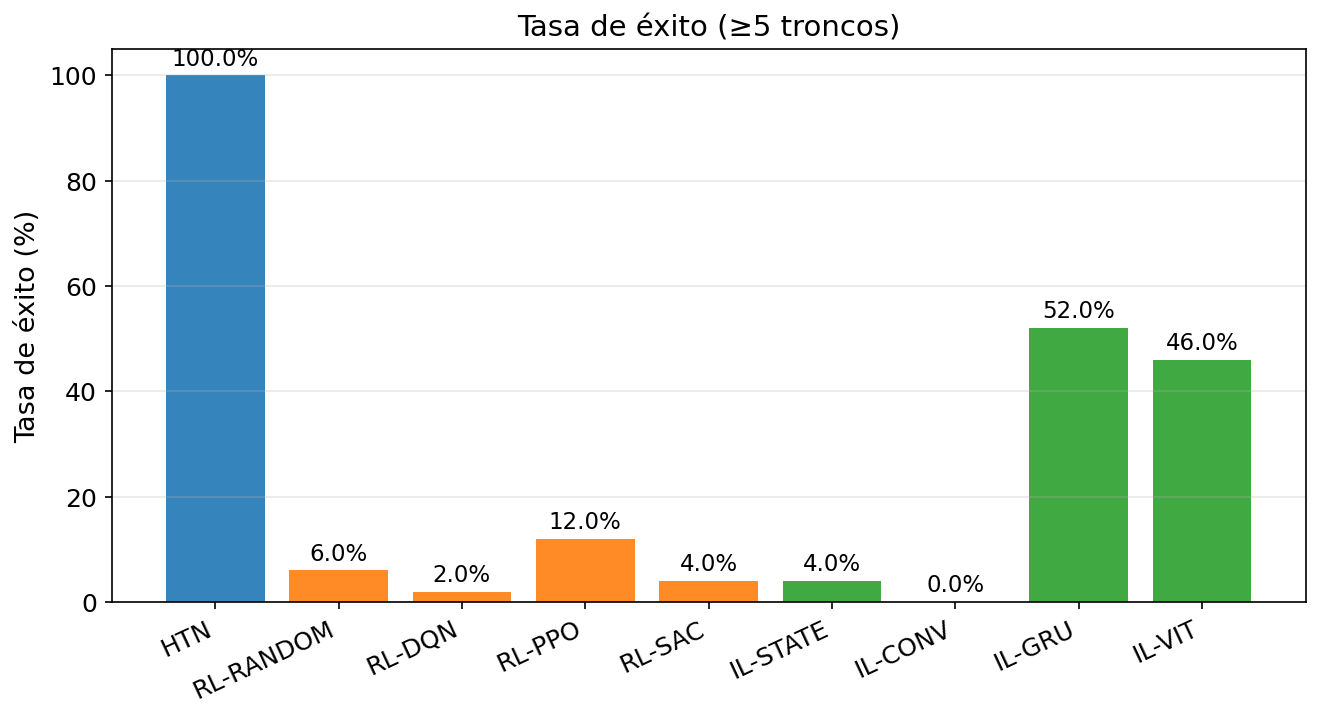
\includegraphics[width=1\textwidth]{imaxes/09_resultados/eval_exito.png}
  }
  \caption[Tasa de éxito por técnica]{Tasa de éxito en entorno bajo la métrica común
  ($\geq \num{5}$ troncos, \num{50} episodios). El \gls{htn} alcanza el objetivo el \qty{100}{\percent} de las veces; 
  entre los agentes entrenados, IL-GRU (\qty{52}{\percent}) e IL-VIT (\qty{46}{\percent}) destacan claramente
  sobre el refuerzo y el agente aleatorio.}
  \label{fig:eval-exito}
\end{figure}

\subsection{Agente Experto}
El \gls{htn} obtiene un \textbf{\qty{100}{\percent} de éxito}, recogiendo exactamente \num{6} troncos por
episodio en \qty{26.7}{\second} de media. El tronco de más sobre el objetivo ($k=\num{5}$) se debe a
que el agente tala el árbol completo antes de reevaluar la condición de parada: la primitiva
de tala rompe todo el tronco de una vez y, en el mundo de evaluación (\gls{semilla} fija), ese árbol
tiene \num{6} bloques. De ahí también su desviación típica nula.
Este resultado era esperable: el planificador opera sobre la información
de la \acrshort{api} y navega de forma óptima con el \gls{pathfinder}
(Capítulo~\ref{chap:iter1}). Su tasa de éxito y eficacia lo convierten en la cota superior 
de la tarea y el límite a alcanzar por el resto de técnicas.

\subsection{Aprendizaje por Imitación}
La \textbf{IL-GRU} es la mejor técnica de todos los agentes
entrenados, con un \textbf{\qty{52}{\percent} de éxito} y una mediana de \num{5} troncos. A diferencia del \gls{htn}, el objetivo se
comprueba una vez por paso de inferencia, de modo que entre comprobaciones el agente puede
recoger varios troncos a la vez; por eso sus episodios exitosos terminan con \num{5}, \num{6} o \num{7}
troncos (Figura~\ref{fig:eval-exito}, página~\pageref{fig:eval-exito}).
La variante \gls{vit} llega a un \qty{46}{\percent}, mientras que las
variantes más simples no consiguen un rendimiento apreciable: solo-estado se queda en el \qty{4}{\percent}
y \gls{convlstm} en el \qty{0}{\percent}. Esto confirma la importancia de la extracción de información de la
imagen en la tarea de imitación. 

Como se menciona en la Sección~\ref{sec:il-sin-exploracion} (página~\pageref{sec:il-sin-exploracion}), el agente aprende
a talar un árbol visible, pero no a encontrarlo. De ahí que falle cerca de la
mitad de los episodios, o bien porque no tiene un árbol delante o porque se pasa de largo y no lo detecta.

\subsection{Aprendizaje por Refuerzo}
El refuerzo desde cero queda muy por debajo respecto a las técnicas de imitación.
El mejor algoritmo es \textbf{PPO} con un
\textbf{\qty{12}{\percent} de éxito}, seguido del agente aleatorio (\qty{6}{\percent}), \gls{sac} (\qty{4}{\percent}) y
\gls{dqn} (\qty{2}{\percent}). El dato más importante es que \gls{dqn} y \gls{sac} no superan al
\textit{\gls{baseline}} aleatorio, indicando que no llegan a consolidar una política útil. 
Solo PPO se separa del \textit{\gls{baseline}}. Sin embargo, cabe mencionar que sí se observan
comportamientos de un funcionamiento correcto, lo que indica que con más episodios (tomando como
referencia \textit{MineRL}~\cite{guss2019minerl}) probablemente se obtendría un rendimiento mucho mejor.

\section{Comparativa Global}
\label{sec:eval-global}
Ordenando las técnicas bajo la métrica común se obtiene la siguiente jerarquía:
\begin{center}
  \resizebox{\textwidth}{!}{$ \displaystyle
    \text{HTN}~(\qty{100}{\percent}) \;\gg\; \text{IL-GRU}~(\qty{52}{\percent}) \approx \text{IL-VIT}~(\qty{46}{\percent}) \;\gg\; \text{PPO}~(\qty{12}{\percent}) \;>\; \text{aleatorio}~(\qty{6}{\percent}) \;>\; \text{SAC},\,\text{DQN}
  $}
\end{center}

Usando esta jerarquía y los resultados mencionados anteriormente, podemos concluir la importancia que
presenta la información del experto a la hora de completar la tarea y la capacidad de extraer información de las imágenes. 
Esta premisa se ve claramente con el rendimiento de las técnicas de imitación, frente a las de refuerzo, cuadruplicando la tasa de éxito de 
su contrapartida, gracias a la información que le proporciona el experto.

Sin embargo, esto no inhabilita la capacidad de aprendizaje del refuerzo, que sí consigue aprender relativamente
la tarea. Durante las ejecuciones de entrenamiento y evaluación sí se observa un comportamiento de
identificación del árbol, navegación hacia él y tala del mismo.
En el Capítulo~\ref{chap:conclusions} se proponen unas líneas de trabajo que combinan 
la información del experto con el refuerzo, para mejorar su rendimiento y eficiencia.

Por último, destacar que, aunque el escenario de evaluación es favorable, los parámetros de
evaluación son exigentes. Con un máximo de \num{200} pasos por episodio,
el agente tiene que ser eficiente en su comportamiento y conseguir talar múltiples troncos. 
Reduciendo el número de troncos objetivo, 
como se observa en la Figura~\ref{fig:eval-exito-umbrales} (página~\pageref{fig:eval-exito-umbrales}), los resultados mejoran considerablemente, aunque
manteniendo la jerarquía de rendimiento mencionada anteriormente.

\begin{figure}[htbp]
  \centering
  \resizebox{\textwidth}{!}{
  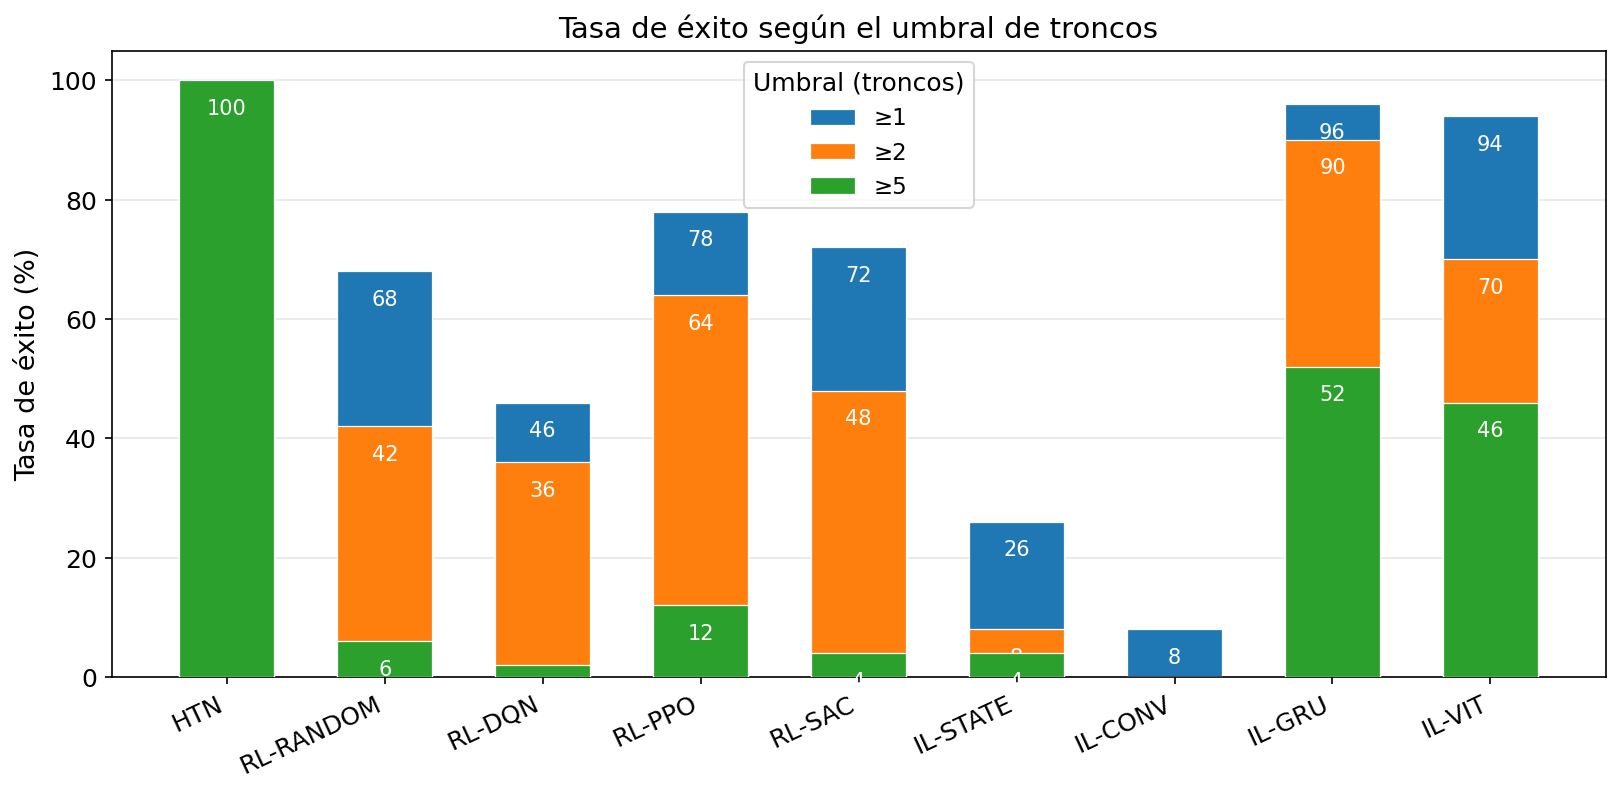
\includegraphics[width=1\textwidth]{imaxes/09_resultados/eval_exito_umbrales_apilado.png}
  }
  \caption[Tasa de éxito según el umbral de troncos]{Tasa de éxito de cada técnica al exigir
  $\geq \num{1}$, $\geq \num{2}$ y $\geq \num{5}$ troncos, superpuestas sobre la misma barra (\num{50} episodios).
  El \gls{htn} mantiene el \qty{100}{\percent} en los tres umbrales; en el resto el éxito decae al subir
  la exigencia, de forma acusada en el refuerzo (PPO: $\num{78}\!\to\!\num{64}\!\to\!\qty{12}{\percent}$) y más contenida
  en IL-GRU ($\num{96}\!\to\!\num{90}\!\to\!\qty{52}{\percent}$).}
  \label{fig:eval-exito-umbrales}
\end{figure}